\documentclass[a4paper]{scrartcl}


\usepackage[utf8]{inputenc}
\usepackage[ngerman]{babel}
\usepackage{enumerate}
\usepackage{tikz}
\usepackage{fancyhdr}
\usepackage{lastpage}
\usepackage{verbatim}

\usepackage{listings}
\setlength{\parindent}{0mm}
\usepackage{graphicx}
\usepackage{amsmath}
\usepackage{algorithm2e}

\pagestyle{fancy}
\fancyhead[L]{SS 2017\\Joshua Hartmann}
\fancyhead[C]{Entwurf und Synthese von Eingebetteten Systemen\\Manfred Opel}
\fancyhead[R]{Blatt 8\\Nicola Staller}

\fancyfoot[L]{}
\fancyfoot[C]{\thepage /\pageref{LastPage}}
\fancyfoot[R]{}

\renewcommand{\textheight}{700px}
\renewcommand{\footskip}{10px}
\newcommand*\xor{\mathbin{\oplus}}
\begin{document}	
\section*{Aufgabe 1: HLS: Ablaufplanung nach ASAP und ALAP}

\begin{enumerate}[(a)]
	\item Datenflussgraph:	
	
	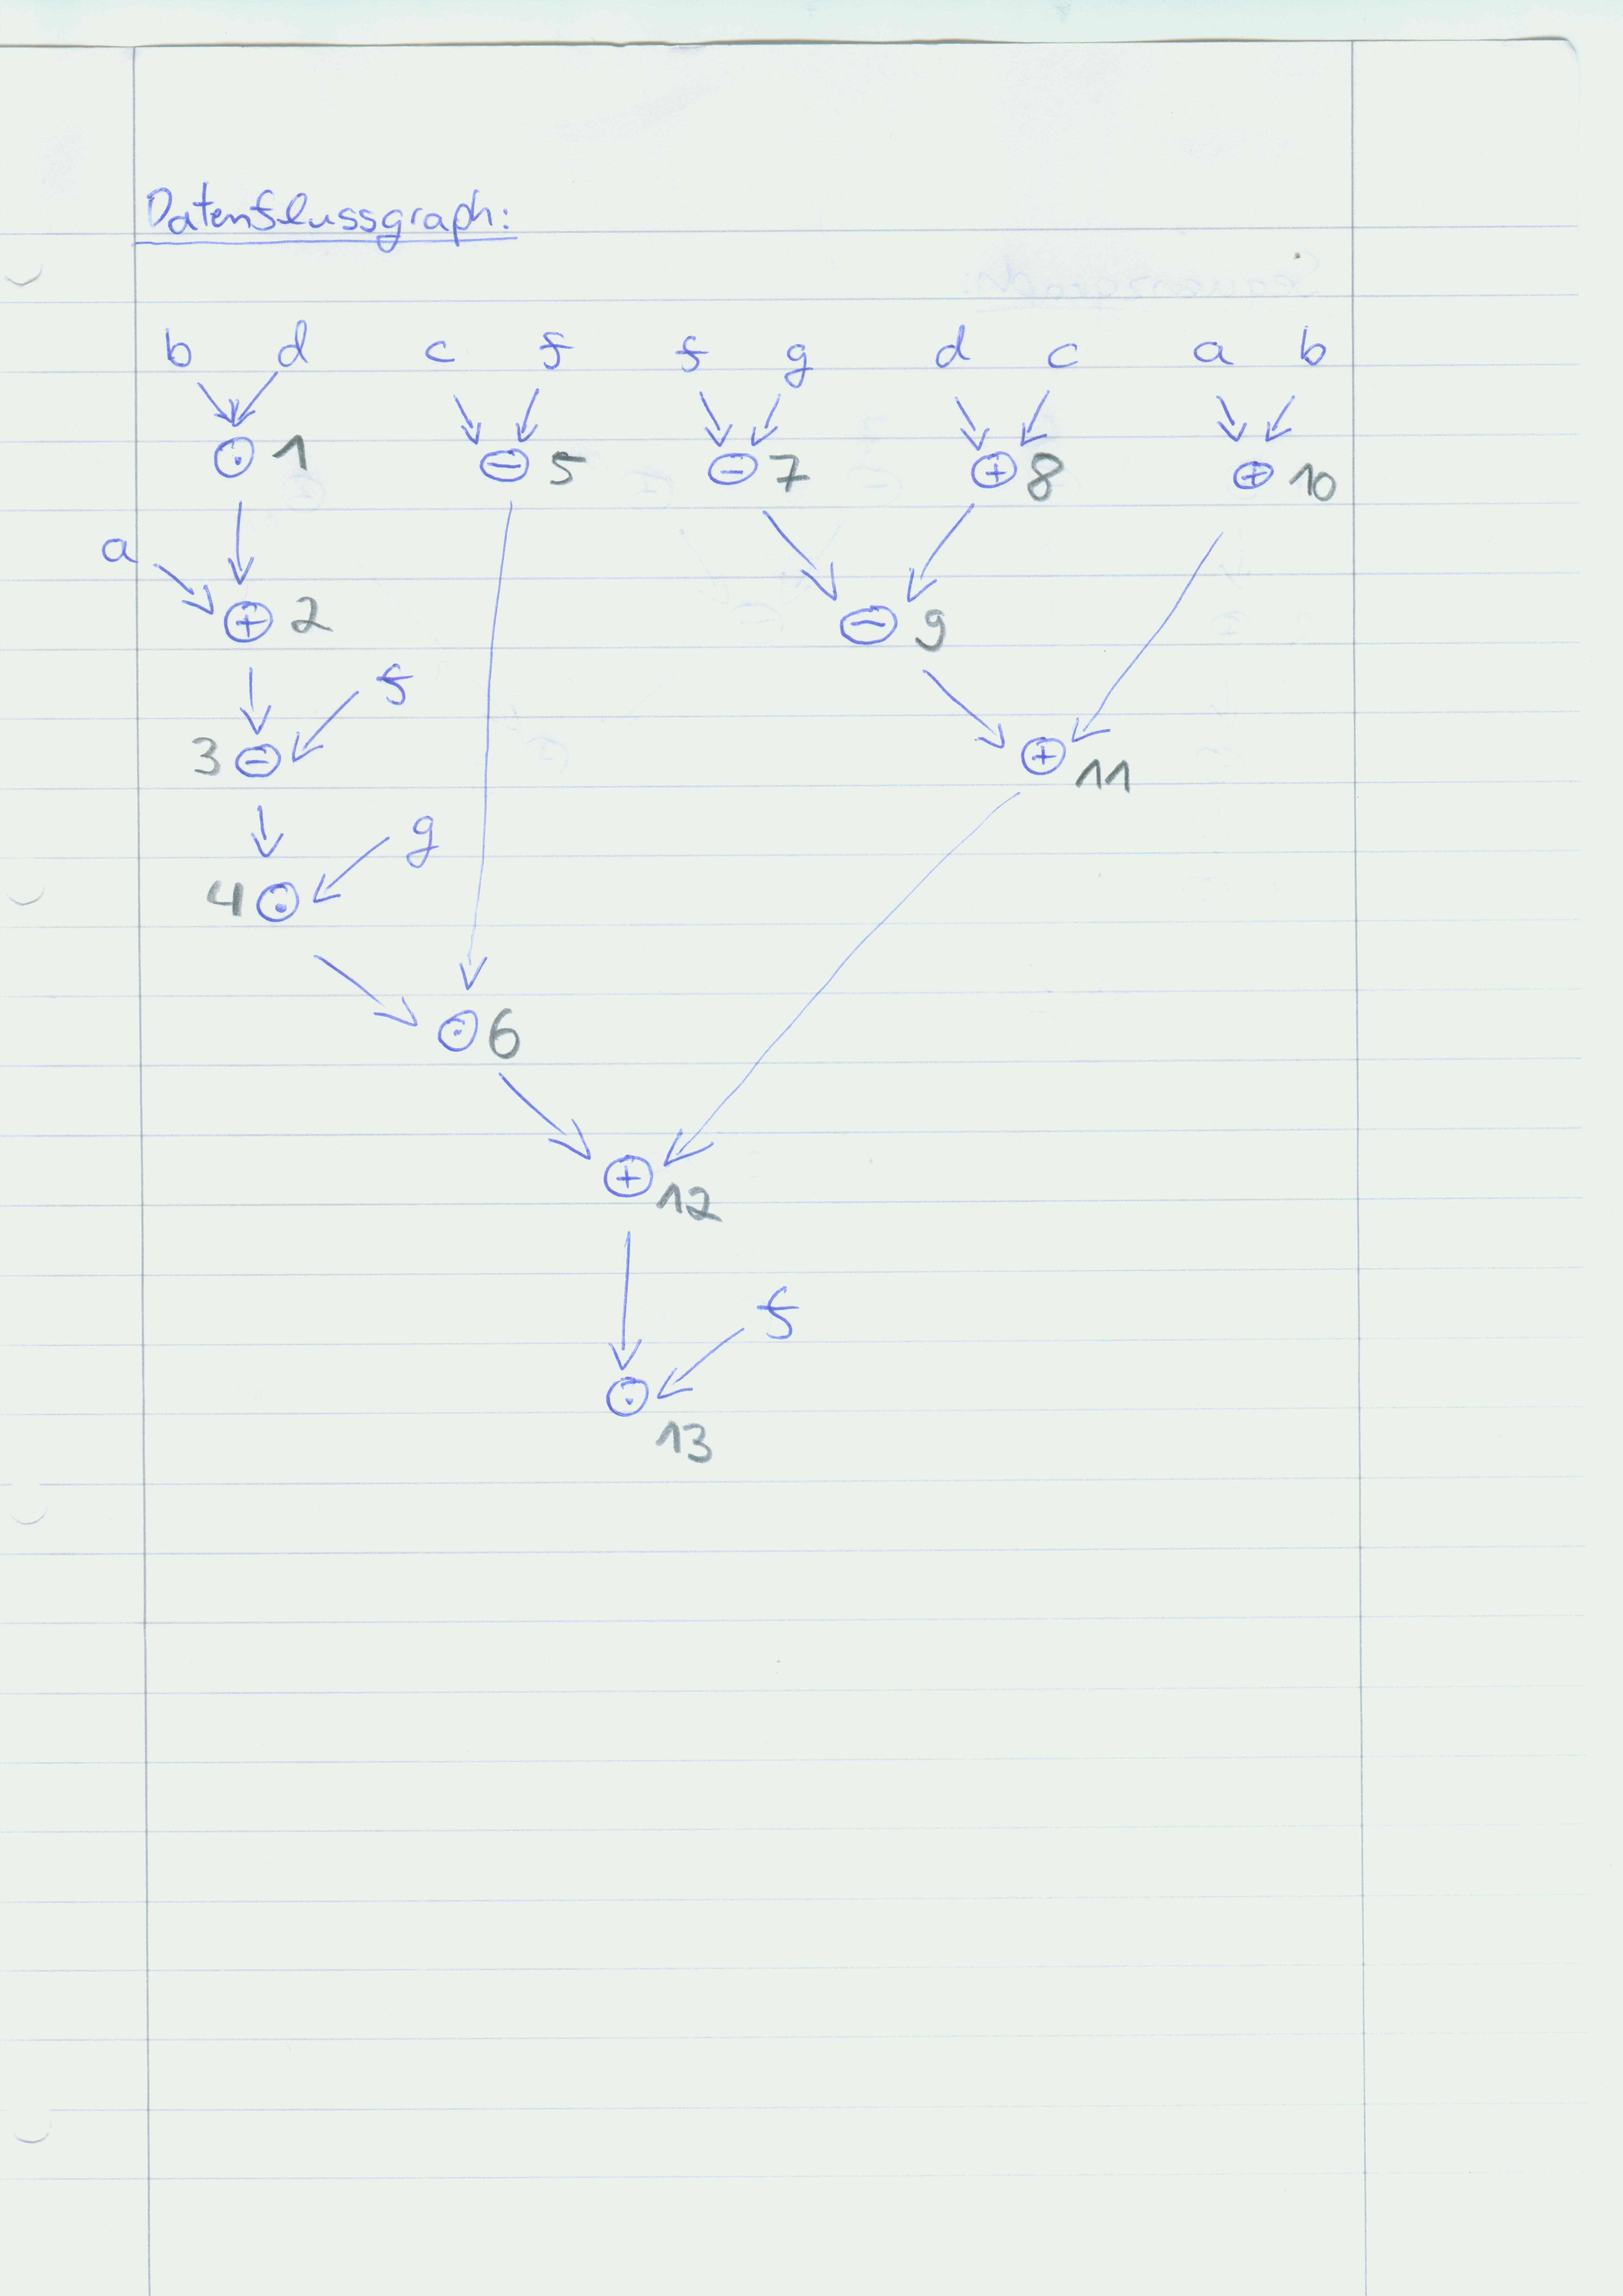
\includegraphics[scale=0.7]{Image121}
	\newpage
	\item Sequenzgraph:
	
	$V = \{1,2,3,4,5,6,7,8,9,10,11,12,13\}$\\
	$E = \{(1,2),(2,3),(3,4),(4,5),(6,5), (7,8),(8,9), (10,8), (11,9), (9,12), (12,13) \}$

	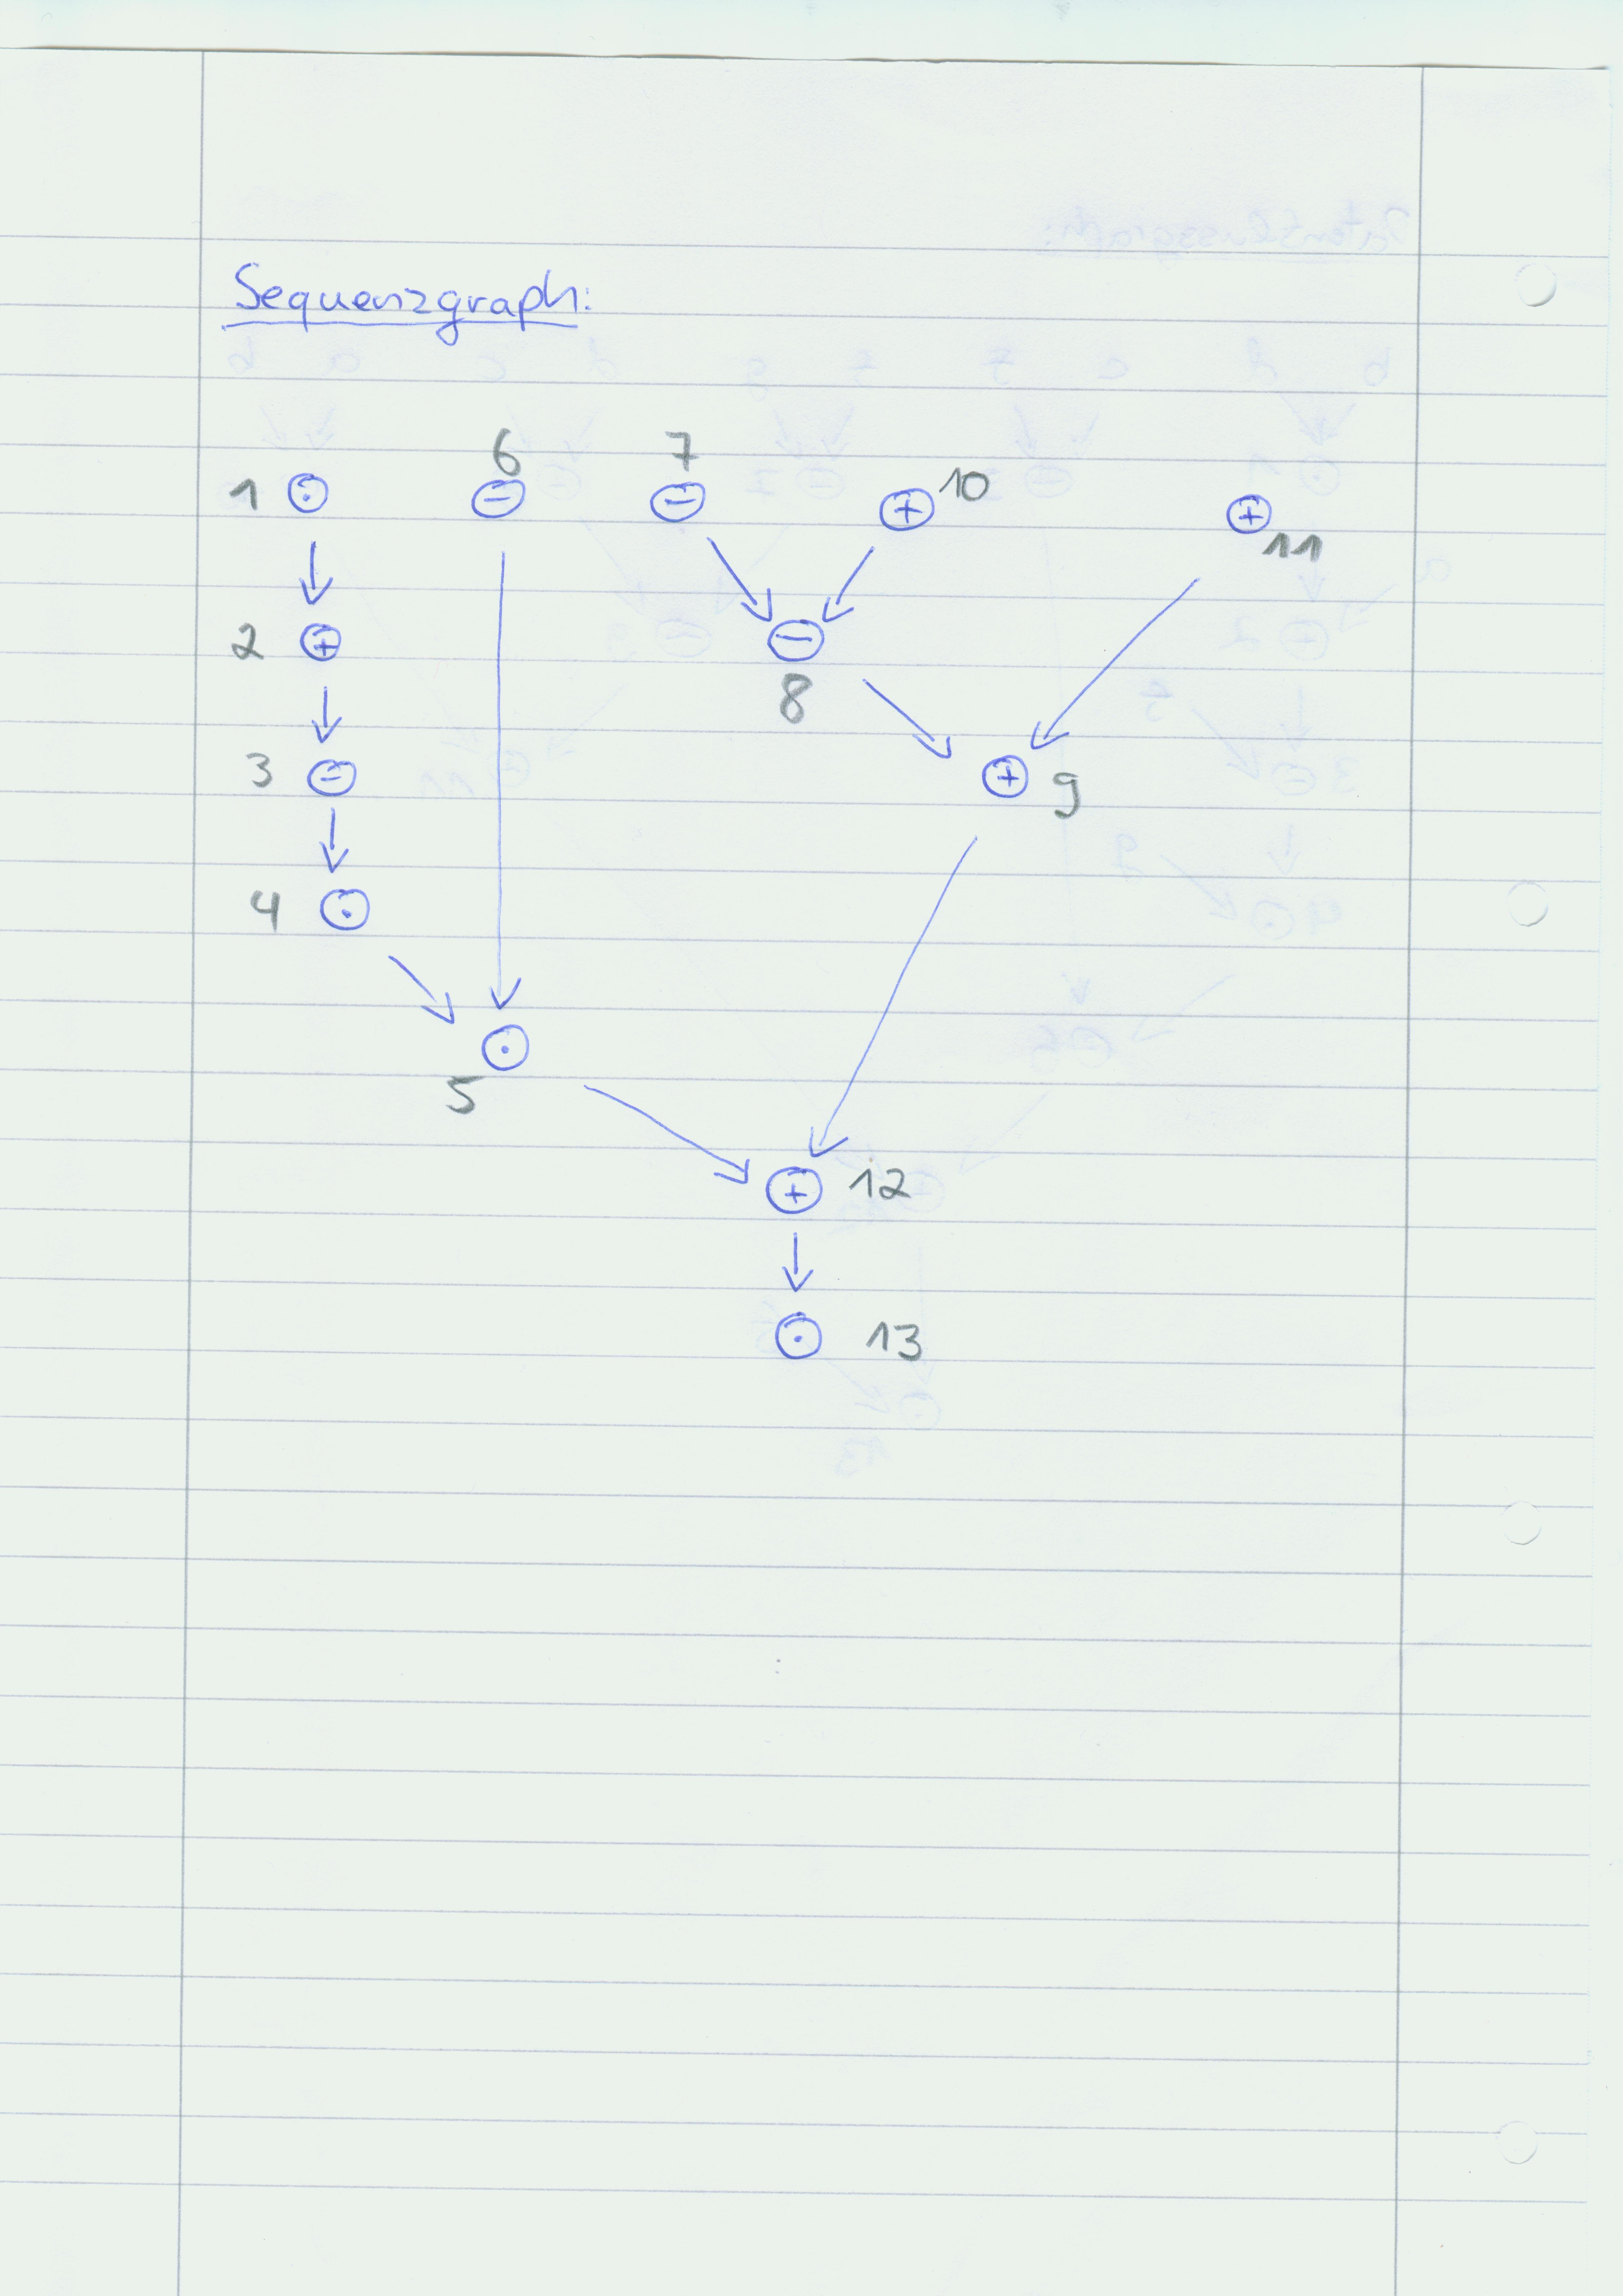
\includegraphics[scale=0.7]{Image122}	
	\newpage
	\item ASAP und ALAP
	
	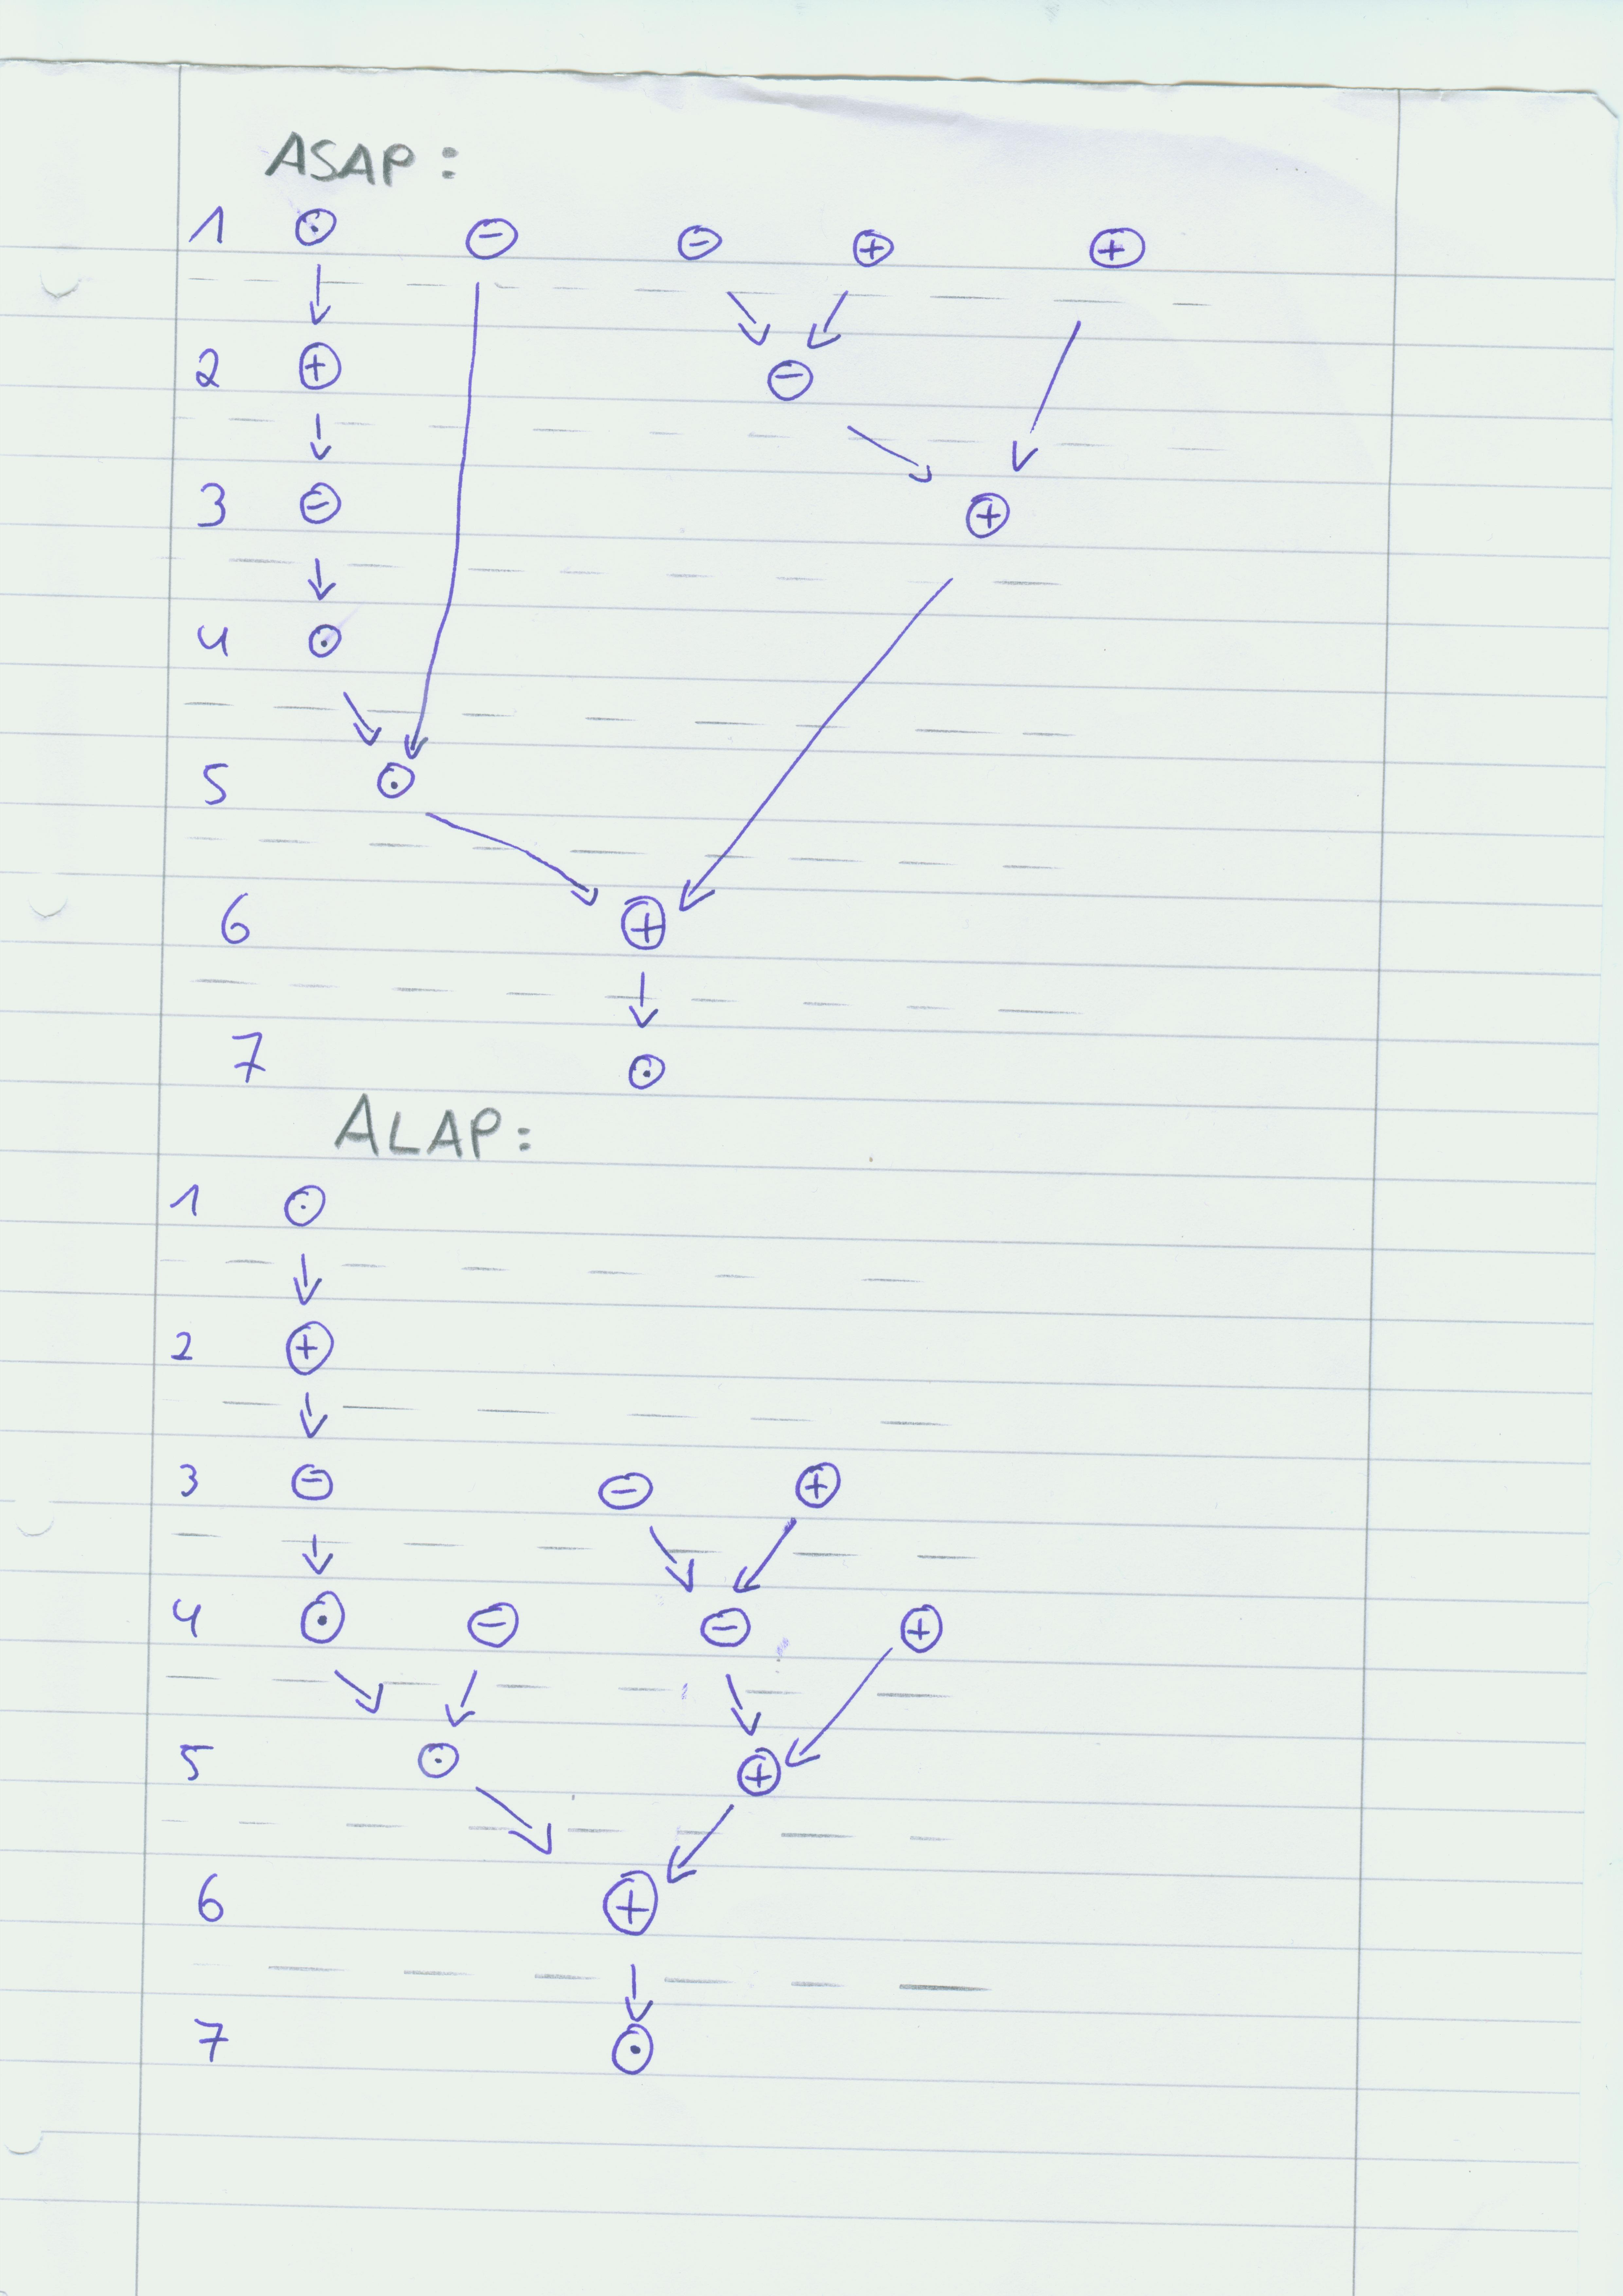
\includegraphics[scale=0.7]{Image123}
	\newpage
	\item Mobilitäten:\\
	\begin{tabular}{c|c}
		Knoten & Mobilität \\ 
		\hline 
		1& 0\\
		2& 0\\
		3& 0\\
		4& 0\\
		5& 0\\
		6& 3\\
		7& 2\\
		8& 2\\
		9& 2\\
		10 & 2\\
		11& 3\\
		12& 0\\
		13& 0\\
	\end{tabular}	
			
	Operationen mit Mobilität 0 liegen auf dem kritischen Pfad und haben deshalb keinen Spielraum, den man in der Optimierung nutzen kann.	
\end{enumerate}

\newpage
\section*{Aufgabe 2: High-Level-Synthese mit Xilinx Vivado HLS}

\begin{enumerate}[(a)]
	\item
	\item \textbf{opcode}, \textbf{in1} und \textbf{in2} entsprechend den Parametern der C-Funktion.\\
	\textbf{ap\_return} entspricht der Rückgabe der C-Funktion.\\
	\textbf{ap\_clk} und \textbf{ap\_reset} sind die Eingange für das Clock bzw Reset Signal, da das Design mehr als ein Takt benötigt.\\
	\textbf{ap\_start} muss auf 1 gesetzt sein, damit das Design mit der Arbeit beginnt.\\
	\textbf{ap\_ready} gibt an, ob das Design bereit ist, neue Eingaben zu verarbeiten.\\
	\textbf{ap\_done} gibt an, ob das Design mit der aktuellen Arbeit fertig ist.\\
	\textbf{ap\_idle} gibt an, ob das Design gerade arbeitet oder idle ist.
	
	Die Erklärungen zu den nicht C-Code spezifischen Ports sind aus dem verlinkten Tutorial ab Seite 69 entnommen.
	\item Der gesamte geschätzte Flächenverbrauch sind 181 Flip-Flops und 248 LUT
	\item Die geschätzte Taktperiode beträgt 5.41ns
	\item In unserem Report findet man nur minimale und maximale Latenzen von 1 bzw 19.\\
	Wenn man in Vivaldo HLS auf Analyse klickt findet man, wie viele Control Steps jede der genannten Operationen braucht. Wir nehmen einfach mal diese Werte als die gesuchten an.\\
	Dann ergeben sich für Addition, Subtraktion und Multiplikation 1 Latenzzyklus und für die Division 19 Latenzzyklen.
	
	\item	
	
	\item Der gesamte Flächenverbrauch beträgt 174 LUTs und 168 FLip-Flops.\\
	Die Werte in Teilaufgabe (c) waren nur Schätzungen auf Grundlage der High Level Synthese. Erst bei der tatsächlichen Implementierung ergeben sich konkrete Werte für den Flächenverbrauch. 
	\item Ja, die Implementierung erfüllt das spezifizierte Timing-Constraint ('All user specified timing constraints are met.')\\
	
	Es ist ein Slack von 17.484ns angegeben. Damit darf die maximale Taktperiode etwa 2.5ns betragen. (Umrechnung in Taktfrequenz wäre eben f = 1/T, aber wir sollen es gleich wieder mit der Periode vergleichen, also gehen wir eher von einem Schreibfehler aus).\\
	Geschätzt wurde dabei eine Taktperiode von 5.41ns, die tatsächliche Implementierung kann also mit einem höheren Takt gefahren werden als ursprünglich angenommen.
\end{enumerate}

	
\end{document}

